%%%%%%%%%%%%%%%%%%%%%%%%%%%%%%%%%%%%%%%%%%%%%%%%%%%%%%%%%%%%%%%%%
% MUW Presentation
% LaTeX Template
% Version 1.0 (27/12/2016)
%
% License:
% CC BY-NC-SA 4.0 (http://creativecommons.org/licenses/by-nc-sa/3.0/)
%
% Created by:
% Nicolas Ballarini, CeMSIIS, Medical University of Vienna
% nicoballarini@gmail.com
% http://statistics.msi.meduniwien.ac.at/
%
% Customized for UAH by:
% David F. Barrero, Departamento de Automática, UAH
%%%%%%%%%%%%%%%%%%%%%%%%%%%%%%%%%%%%%%%%%%%%%%%%%%%%%%%%%%%%%%%%%

\documentclass[10pt,compress]{beamer} % Change 10pt to make fonts of a different size
\mode<presentation>

\usepackage[spanish]{babel}
\usepackage{fontspec}
\usepackage{tikz}
\usepackage{etoolbox}
\usepackage{xcolor}
\usepackage{xstring}
\usepackage{listings}

% Custom packages
\usepackage{tikz}
\usepackage{pgfplots}
\def\layersep{2.5cm}
\usetikzlibrary{matrix,chains,positioning,decorations.pathreplacing,arrows}

\definecolor{dkgreen}{rgb}{0,0.6,0}
\definecolor{gray}{rgb}{0.5,0.5,0.5}
\definecolor{mauve}{rgb}{0.58,0,0.82}
 

\usetheme{UAH}
\usecolortheme{UAH}
\setbeamertemplate{navigation symbols}{} 
\setbeamertemplate{caption}[numbered]

%%%%%%%%%%%%%%%%%%%%%%%%%%%%%%%%%%%%%%%%%%%%%%%%%%%%%%%%%%%%%%%%%
%% Presentation Info
\title[Search algorithm]{Solving Problems by Searching}
\author{\asignatura\\\carrera}
\institute{}
\date{Departamento de Automática}
%%%%%%%%%%%%%%%%%%%%%%%%%%%%%%%%%%%%%%%%%%%%%%%%%%%%%%%%%%%%%%%%%


%%%%%%%%%%%%%%%%%%%%%%%%%%%%%%%%%%%%%%%%%%%%%%%%%%%%%%%%%%%%%%%%%
%% Descomentar para habilitar barra de navegación superior
\setNavigation
%%%%%%%%%%%%%%%%%%%%%%%%%%%%%%%%%%%%%%%%%%%%%%%%%%%%%%%%%%%%%%%%%

%%%%%%%%%%%%%%%%%%%%%%%%%%%%%%%%%%%%%%%%%%%%%%%%%%%%%%%%%%%%%%%%%
%% Configuración de logotipos en portada
%% Opacidad de los logotipos
\newcommand{\opacidad}{1}
%% Descomentar para habilitar logotipo en pié de página de portada
\renewcommand{\logoUno}{Images/isg.png}
%% Descomentar para habilitar logotipo en pié de página de portada
%\renewcommand{\logoDos}{Images/CCLogo.png}
%% Descomentar para habilitar logotipo en pié de página de portada
%\renewcommand{\logoTres}{Images/ALogo.png}
%% Descomentar para habilitar logotipo en pié de página de portada
%\renewcommand{\logoCuatro}{Images/ELogo.png}
%%%%%%%%%%%%%%%%%%%%%%%%%%%%%%%%%%%%%%%%%%%%%%%%%%%%%%%%%%%%%%%%%

%%%%%%%%%%%%%%%%%%%%%%%%%%%%%%%%%%%%%%%%%%%%%%%%%%%%%%%%%%%%%%%%%
%% FOOTLINE
%% Comment/Uncomment the following blocks to modify the footline
%% content in the body slides. 


%% Option A: Title and institute
\footlineA
%% Option B: Author and institute
%\footlineB
%% Option C: Title, Author and institute
%\footlineC
%%%%%%%%%%%%%%%%%%%%%%%%%%%%%%%%%%%%%%%%%%%%%%%%%%%%%%%%%%%%%%%%%

\begin{document}

%%%%%%%%%%%%%%%%%%%%%%%%%%%%%%%%%%%%%%%%%%%%%%%%%%%%%%%%%%%%%%%%%
% Use this block for a blue title slide with modified footline
{\titlepageBlue
    \begin{frame}
        \titlepage
    \end{frame}
}

\institute{\asignatura}

\begin{frame}[plain]{}
   \begin{block}{Objectives}
      \begin{enumerate}
         \item Understand the role of search in AI
         \item Describe the importance of trees in search
         \item Express AI problems in terms of search
         \item Apply classical search algorithms
      \end{enumerate} 
   \end{block}

   \begin{block}{Bibliography}
	\begin{itemize}
        \item S. Russell and P. Norvig. Chapter 3, Solving Problems by Searching. \textit{Artificial Intelligence: A Modern Approach}. Pearson. 2017
	\end{itemize}
   \end{block}
\end{frame}

{
\disableNavigation{white}
\begin{frame}[shrink]{Table of Contents}
 \frametitle{Table of Contents}
 \tableofcontents
  % You might wish to add the option [pausesections]
\end{frame}
}

\section{Introduction}

\begin{frame}{Introduction}{Agents}
    \begin{columns}
 	   \column{.50\textwidth}
        \begin{block}{Agent}
        An agent is anything that can be viewed as perceiving its environment through sensors and acting through actuators
        \end{block}

 	   \column{.50\textwidth}
        \begin{center}
	        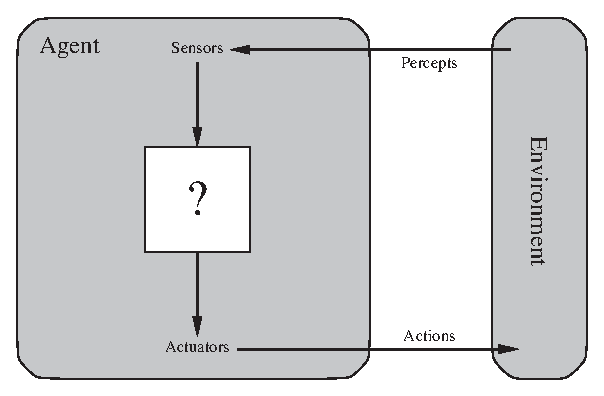
\includegraphics[width=0.9\linewidth]{figs/agent-environment.eps}\\
	        \tiny{\href{http://aima.cs.berkeley.edu/index.html}{(Source)}}
	    \end{center}

	\end{columns}

    \begin{itemize}
        \item Agents is a research field in AI by its own 
            \begin{itemize}
                \item ... with its own definition of agent (caution!)
            \end{itemize}
        \item We use this term to abstract the implementation
    \end{itemize}
\end{frame}

\subsection{Types of problems}
\begin{frame}{Introduction}{Types of problems}
    Types of problems depending on ...
	\begin{itemize}
        \item Knowledge
            \begin{itemize}
                \item[-] Observable or Non-observable or Partially observable
            \end{itemize}
        \item Outcome
            \begin{itemize}
                \item[-] Deterministic or Stochastic
            \end{itemize}
        \item Actions
            \begin{itemize}
                \item[-] Discrete or Continous
            \end{itemize}
        \item Time-variance
            \begin{itemize}
                \item[-] Static or Dynamic
            \end{itemize}
	\end{itemize}
    We assume static, observable, discrete and deterministic problems
\end{frame}

\begin{frame}[fragile]{Introduction}{Types of problems (II)}
    \begin{exampleblock}{Determine problem type}
       \begin{columns}
 	       \column{.50\textwidth}
           \centering Chess\\
           \medskip
	        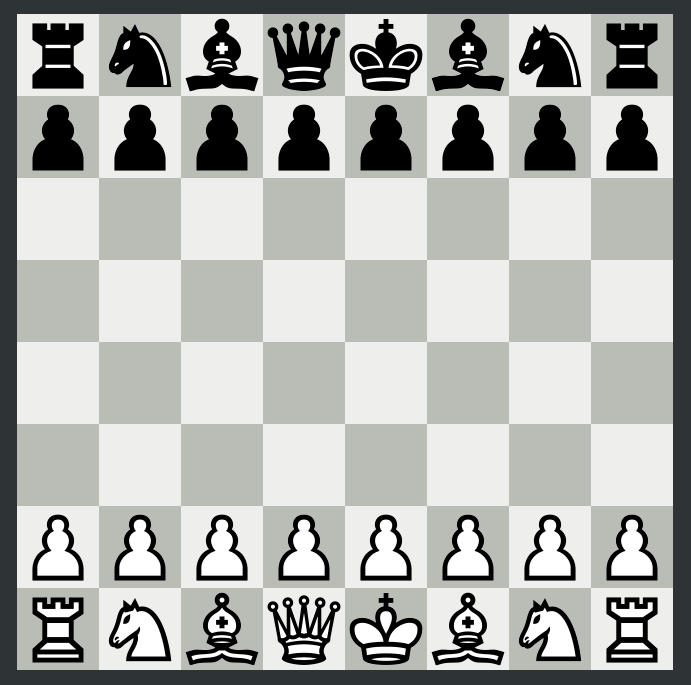
\includegraphics[width=0.75\linewidth]{figs/chess.png}\\

 	       \column{.50\textwidth}
           \centering League of Legends\\
           \medskip
	        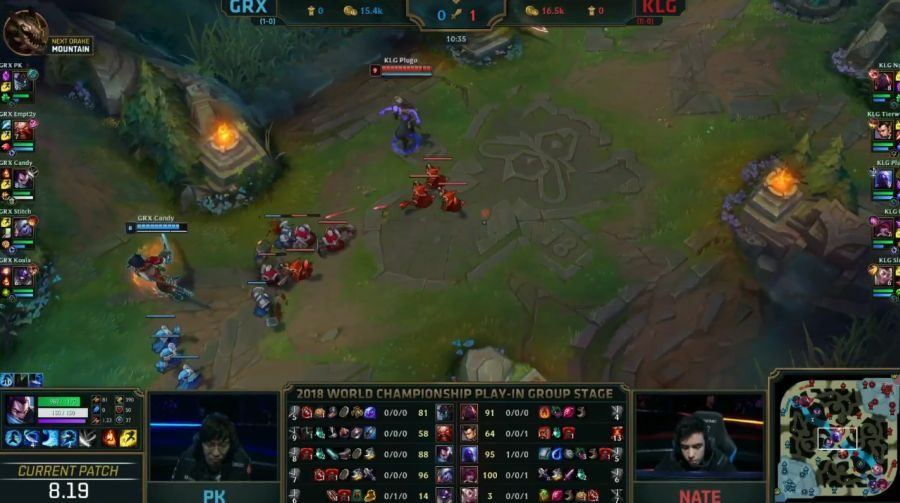
\includegraphics[width=0.75\linewidth]{figs/lol.jpg}\\
        \end{columns}
        \medskip
        Observable or non-observable, deterministic or stochastic, discrete or continous, static or dynamic?
    \end{exampleblock}
\end{frame}

\subsection{Problem components}
\begin{frame}{Introduction}{Problem components (I)}
	\begin{itemize}
        \item[Initial state] State where the search begins
        \item[Actions] XXX
        \item[Transition model] XXX
        \item[Goal test] XXX
        \item[Path cost] Process of looking a sequence of actions that reach the goal
	\end{itemize}
    \alert{Search} is the process of looking a sequence of actions that reach the goal
\end{frame}

\begin{frame}{Introduction}{Problem components (II)}
    \begin{center}
	    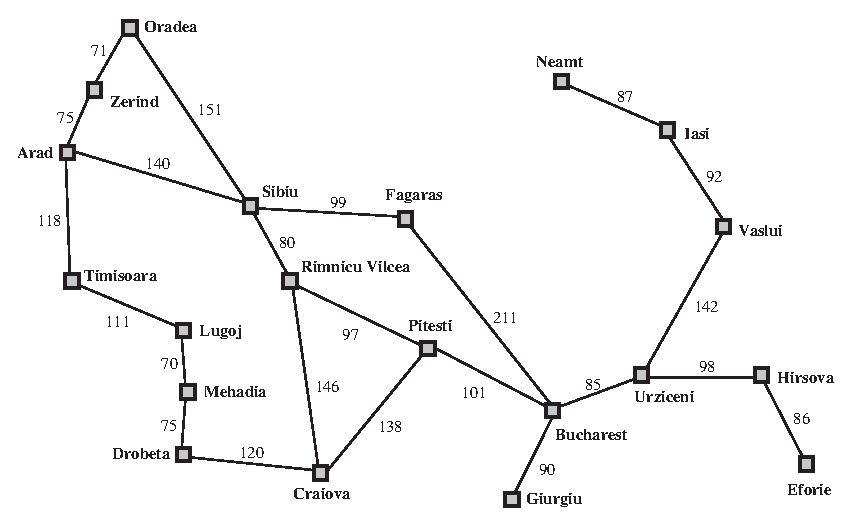
\includegraphics[width=0.7\linewidth]{figs/romania-distances.eps}\\
	    \tiny{\href{http://aima.cs.berkeley.edu/index.html}{(Source)}}
	\end{center}
    \begin{exampleblock}{Problem: Move from Arad to Bucharest}
        Initial state? Goal? Actions? Transition model? Goal test? Path cost?
    \end{exampleblock}
\end{frame}

\subsection{Toy problems}
\begin{frame}[fragile]{Introduction}{Toy problems (I): Vacuum world}
       \begin{columns}
 	       \column{.60\textwidth}
	            \centering 
                \onslide<1> 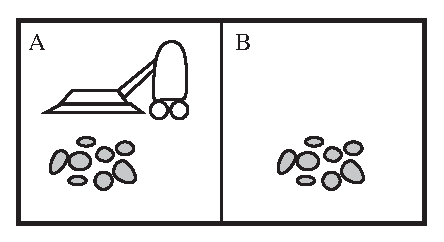
\includegraphics[width=\linewidth]{figs/vacuum2-environment.eps}\\
	            \tiny{\href{http://aima.cs.berkeley.edu/index.html}{(Source)}}

 	       \column{.40\textwidth}
                \begin{exampleblock}{Problem: Clean rooms}
                    \begin{itemize}
                    \item[-] State? $\rightarrow$ 
                    \item[-] Initial state? $\rightarrow$ 
                    \item[-] Goal? $\rightarrow$ 
                    \item[-] Actions? $\rightarrow$ 
                    \item[-] Transition model? $\rightarrow$ 
                    \item[-] Goal test? $\rightarrow$ 
                    \item[-] Path cost? $\rightarrow$
                    \end{itemize}
                \end{exampleblock}
      \end{columns}
\end{frame}

\begin{frame}[fragile]{Introduction}{Toy problems (I): Vacuum world}
       \begin{columns}
 	       \column{.60\textwidth}
	           \centering 
               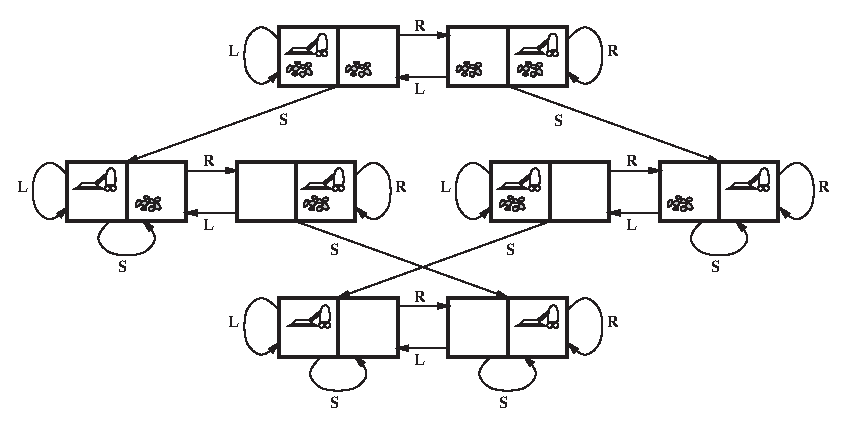
\includegraphics[width=\linewidth]{figs/vacuum2-state-space.eps}\\
	           \tiny{\href{http://aima.cs.berkeley.edu/index.html}{(Source)}}

 	       \column{.40\textwidth}
                \begin{exampleblock}{Problem: Clean rooms}
                    \begin{itemize}
                    \item[-] State? $\rightarrow$ \textit{Dirt and location}
                    \item[-] Initial state? $\rightarrow$ \textit{All dirt, Left}
                    \item[-] Goal? $\rightarrow$ \textit{No dirt, any location}
                    \item[-] Actions? $\rightarrow$ \textit{Left, Right, Suck}
                    \item[-] Transition model? $\rightarrow$ \textit{See figure}
                    \item[-] Goal test? $\rightarrow$ \textit{No dirt, any location}
                    \item[-] Path cost? $\rightarrow$ \textit{1 per action}
                    \end{itemize}
                \end{exampleblock}
      \end{columns}
\end{frame}

\begin{frame}{Introduction}{Toy problems (II): 8-puzzle}
       \begin{columns}
 	       \column{.60\textwidth}
	            \centering 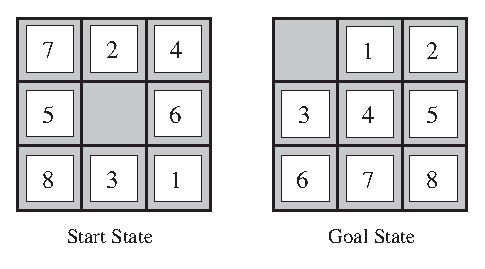
\includegraphics[width=\linewidth]{figs/8puzzle.eps}\\
	            \tiny{\href{http://aima.cs.berkeley.edu/index.html}{(Source)}}
 	       \column{.40\textwidth}
                \begin{exampleblock}{Problem: Solve 8-puzzle}
                    \begin{itemize}
                    \item[-] State? $\rightarrow$ 
                    \item[-] Initial state? $\rightarrow$ 
                    \item[-] Goal? $\rightarrow$ 
                    \item[-] Actions? $\rightarrow$ 
                    \item[-] Transition model? $\rightarrow$ 
                    \item[-] Goal test? $\rightarrow$ 
                    \item[-] Path cost? $\rightarrow$
                    \end{itemize}
                \end{exampleblock}
      \end{columns}
\end{frame}

\begin{frame}{Introduction}{Toy problems (II): 8-puzzle}
       \begin{columns}
 	       \column{.60\textwidth}
	            \centering 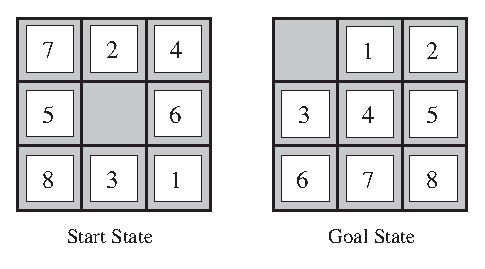
\includegraphics[width=\linewidth]{figs/8puzzle.eps}\\
	            \tiny{\href{http://aima.cs.berkeley.edu/index.html}{(Source)}}
 	       \column{.40\textwidth}
                \begin{exampleblock}{Problem: Solve 8-puzzle}
                    \begin{itemize}
                    \item[-] State? $\rightarrow$ \textit{Location of tiles}
                        \begin{itemize}
                            \item[] $9!/2 = 181,440$ states
                        \end{itemize}
                    \item[-] Initial state? $\rightarrow$ \textit{Any}
                    \item[-] Goal? $\rightarrow$ \textit{See figure}
                    \item[-] Actions? $\rightarrow$ \textit{Left, Right, Up, Down}
                    \item[-] Transition model? $\rightarrow$ Complex graph
                    \item[-] Goal test? $\rightarrow$ \textit{Goal state}
                    \item[-] Path cost? $\rightarrow$ \textit{1 per move}
                    \end{itemize}
                \end{exampleblock}

      \end{columns}
\end{frame}

\begin{frame}{Introduction}{Toy problems (III): 8-queens}
       \begin{columns}
 	       \column{.60\textwidth}
	            \centering 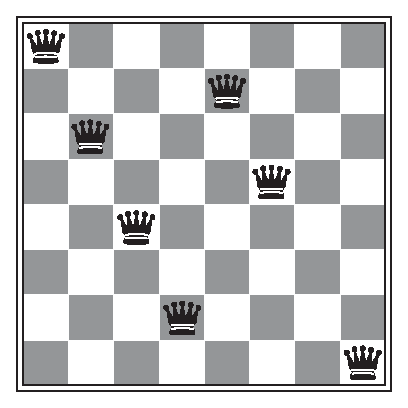
\includegraphics[width=\linewidth]{figs/8queens.eps}\\
	            \tiny{\href{http://aima.cs.berkeley.edu/index.html}{(Source)}}
 	       \column{.40\textwidth}
                \begin{exampleblock}{Problem: Place 8 queens no queen attacks any other}
                State?\\
                Initial state? \\
                Goal? \\
                Actions? \\ 
                Transition model? \\
                Goal test? \\
                Path cost?\\
                \end{exampleblock}
      \end{columns}
\end{frame}

\begin{frame}{Introduction}{Toy problems (III): 8-queens}
       \begin{columns}
 	       \column{.60\textwidth}
	            \centering 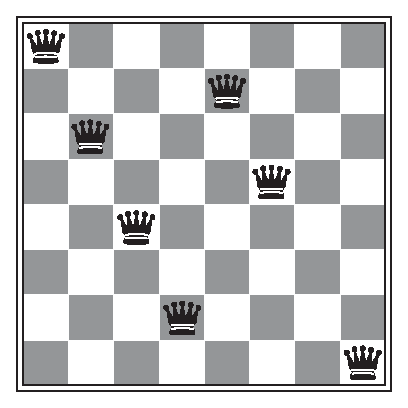
\includegraphics[width=\linewidth]{figs/8queens.eps}\\
	            \tiny{\href{http://aima.cs.berkeley.edu/index.html}{(Source)}}
 	       \column{.40\textwidth}
                \begin{exampleblock}{Problem: Place 8 queens no queen attacks any other}
                    \begin{itemize}
                    \item[-] State? $\rightarrow$ \textit{Any arrangement of 0 to 8 queens}
                    \item[-] Initial state? $\rightarrow$ \textit{Empty board}
                    \item[-] Goal? $\rightarrow$ \textit{See figure}
                    \item[-] Actions? $\rightarrow$ \textit{Add queen to empty square}
                    \item[-] Transition model? $\rightarrow$ Complex graph
                    \item[-] Goal test? $\rightarrow$ \textit{8 queens on board, none attacked}
                    \item[-] Path cost? $\rightarrow$ \textit{1 per move}
                    \end{itemize}
                \end{exampleblock}
      \end{columns}
\end{frame}

\subsection{Real world problems}
\begin{frame}{Introduction}{Real world problems (I): Robotic assembly}
       \begin{columns}
 	       \column{.60\textwidth}
	            \centering 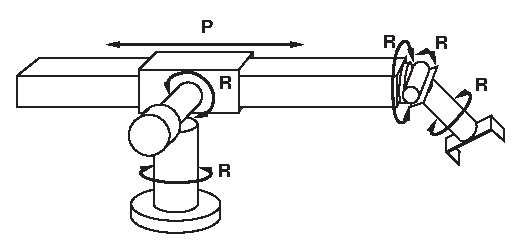
\includegraphics[width=\linewidth]{figs/stanford-arm.eps}\\
	            \tiny{\href{http://aima.cs.berkeley.edu/index.html}{(Source)}}
 	       \column{.40\textwidth}
                \begin{exampleblock}{Problem: Place 8 queens no queen attacks any other}
                State?\\
                Initial state? \\
                Goal? \\
                Actions? \\ 
                Transition model? \\
                Goal test? \\
                Path cost?\\
                \end{exampleblock}
      \end{columns}
\end{frame}

\begin{frame}{Introduction}{Real world problems (I): Robotic assembly}
       \begin{columns}
 	       \column{.60\textwidth}
	            \centering 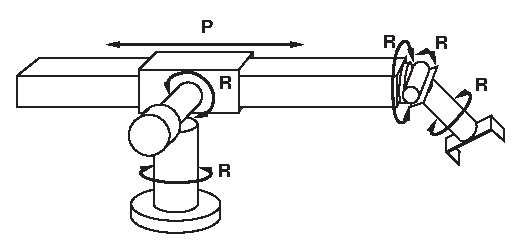
\includegraphics[width=\linewidth]{figs/stanford-arm.eps}\\
	            \tiny{\href{http://aima.cs.berkeley.edu/index.html}{(Source)}}
 	       \column{.40\textwidth}
                \begin{exampleblock}{Problem: Robotic assembly}
                    \begin{itemize}
                    \item[-] State? $\rightarrow$ \textit{Real-valued coordinates of robot joint angles}
                    \item[-] Actions? $\rightarrow$ \textit{Continuous motions of joints}
                    \item[-] Goal test? $\rightarrow$ \textit{Complete assembly}
                    \item[-] Path cost? $\rightarrow$ \textit{Time to complete}
                    \end{itemize}
                \end{exampleblock}

      \end{columns}
\end{frame}

\begin{frame}{Introduction}{Real world problems (II): Travel Salesman Problem (TSP)}
       \begin{columns}
 	       \column{.40\textwidth}
                TSP formulation
                \begin{itemize}
                    \item A travel salesman must visit a set of cities
                    \item One time in each city
                    \item Find the shortest route
                \end{itemize}

                TSP is a very big problem in AI!
                \begin{itemize}
                    \item Many real world applications
                    \item NP-hard problem
                \end{itemize}

 	       \column{.60\textwidth}
                \begin{center}
                    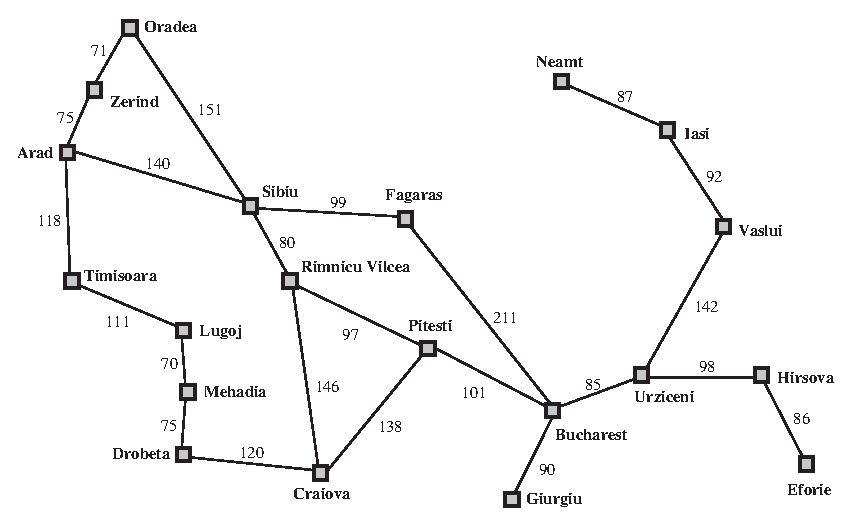
\includegraphics[width=\linewidth]{figs/romania-distances.eps}\\
                    \tiny{\href{http://aima.cs.berkeley.edu/index.html}{(Source)}}
                \end{center}
      \end{columns}
\end{frame}

\section{Search strategy}

\begin{frame}{Search strategy (I)}
    In general ...
	    \begin{itemize}
    	    \item Each problem has a search graph, or \alert{state space}
        	\item Searching means finding a path from the initial state to a goal state
    	\end{itemize}

    Basic idea
        \begin{itemize}
            \item Explore search space
            \item Generate a search tree \alert{expanding states}
        \end{itemize}

    A \alert{search strategy} is defined by picking the order of node exansion
        \begin{itemize}
            \item Uninformed search: Only uses the problem definition
            \item Informed search: Uses problem-specific knowledge
        \end{itemize}
\end{frame}

\begin{frame}{Search strategy (II)}
    Search strategies are evaluated along the following dimensions
	    \begin{itemize}
    	    \item Completeness
        	\item Time complexity
            \item Space complexity
            \item Optimality
    	\end{itemize}

    Time and space are measured in terms of 
        \begin{itemize}
            \item b: Maximum branching factor
            \item d: Depth of the least-cost solution
            \item m: Maximum depth of the state space
        \end{itemize}
\end{frame}

%\section{Uninformed search}
%\subsection{Introduction}

%\begin{frame}{Uninformed search}{Introduction}
%    Uninformed search algorithms
%    \begin{itemize}
%        \item Breadth-first search (\textit{búsqueda en anchura})
%        \item Uniform-cost search (\textit{búsqueda de coste uniforme})
%        \item Depth-first search (\textit{búsqueda en profundidad})
%        \item Depth-limited search (\textit{búsqueda en profundidad limitada})
%        \item Iterative deepening search (\textit{búsqueda de profundización iterativa})
%    \end{itemize}
%\end{frame}

\subsection{Breadth-first search}

\begin{frame}{Uninformed search}{Breadth-first search (I)}
      Expand shallowest unexpanded node
      \begin{itemize}
        \item Implemented with a FIFO queue (First-In First-Out)
      \end{itemize}

      \bigskip 

      \begin{center}
          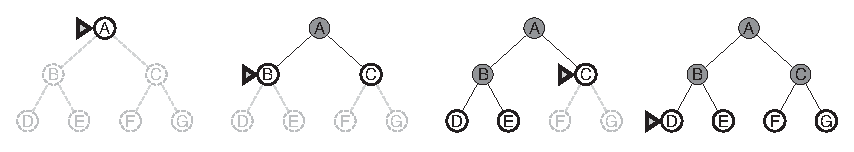
\includegraphics[width=\linewidth]{figs/bfs-progress.eps}\\
          \tiny{\href{http://aima.cs.berkeley.edu/index.html}{(Source)}}
      \end{center}
\end{frame}

\begin{frame}{Uninformed search}{Breadth-first search (II)}
      \begin{center}
          \setlength{\fboxrule}{0pt}
          \fbox{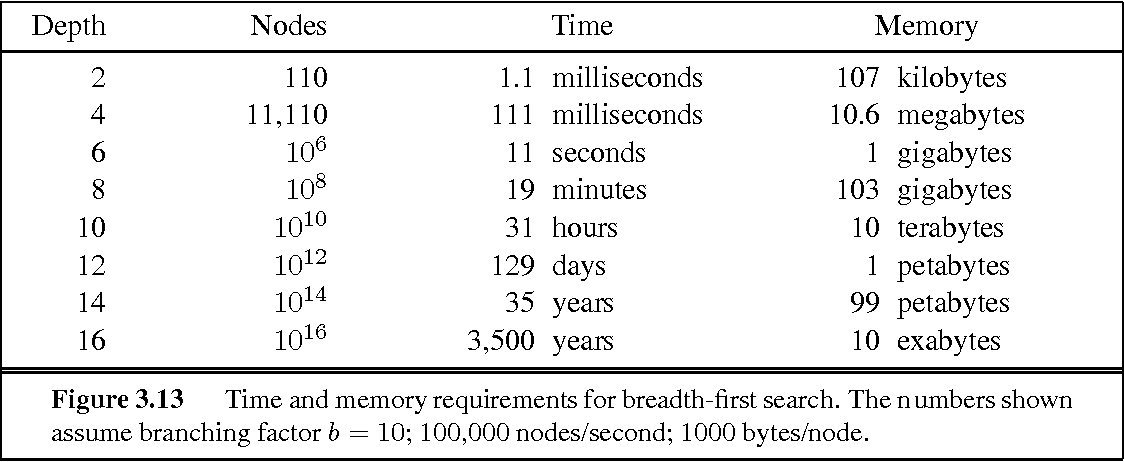
\includegraphics[natwidth=1124bp,natheight=462bp, width=0.7\linewidth]{figs/20-Figure3.13-1.png}} \\
          %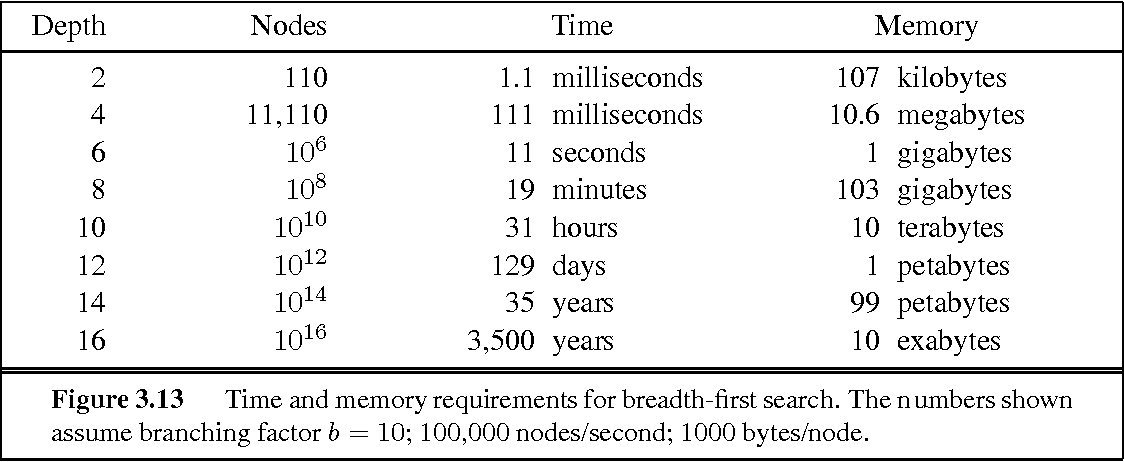
\includegraphics[natwidth=1124, natwidth=462]{figs/20-Figure3.13-1.png}\\
          \tiny{\href{http://aima.cs.berkeley.edu/index.html}{(Source)}}
      \end{center}

      \bigskip
      Properties of breadth-first search
      \begin{itemize}
        \item Completeness: Yes
        \item Time complexity: $O(b^{d+1})$
        \item Space complexity: $O(b^{d+1})$
        \item Optimality: Yes (if cost = 1 per step)
      \end{itemize}
      Space is the biggest problem (more than time)
\end{frame}

\subsection{Uniform-cost search}

\begin{frame}{Uninformed search}{Uniform-cost search (I)}
    Expand least-cost unexpanded node
    \begin{itemize}
        \item Implemented with a queue ordered by path cost
    \end{itemize}

    \begin{columns}
 	       \column{.50\textwidth}
                \setlength{\fboxrule}{0pt}
                \fbox{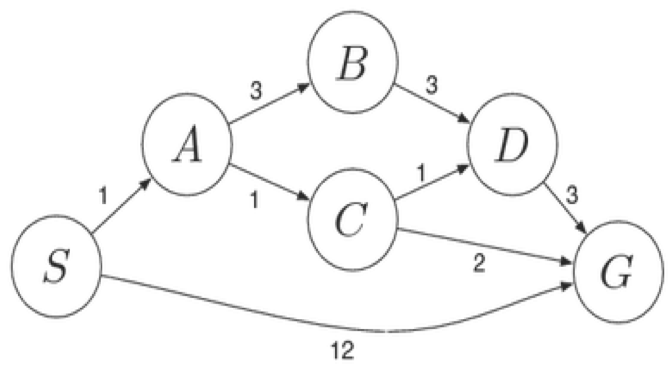
\includegraphics[width=\linewidth]{figs/Grafo1.png}} 
 	       \column{.50\textwidth}
                \setlength{\fboxrule}{0pt}
                \fbox{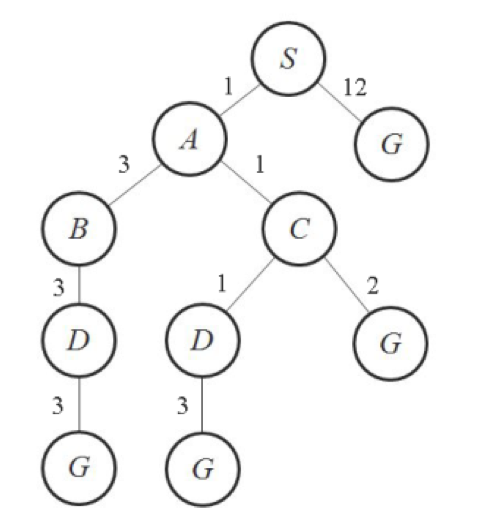
\includegraphics[width=0.7\linewidth]{figs/Grafo2.png}} 
    \end{columns}
\end{frame}

\begin{frame}[fragile]{Uninformed search}{Uniform-cost search (II)}
    \begin{exampleblock}{Uniform-cost example}
    \small{
    Initialization: $\{[S, 0]\}$\\
    Iter. 1: $\{[S \rightarrow A, 1], [S \rightarrow G, 12]\}$\\
    Iter. 2: $\{[S \rightarrow A \rightarrow C, 2], [S \rightarrow A \rightarrow B, 4], [S \rightarrow G, 12]\}$\\
    Iter. 3: $\{[S \rightarrow A \rightarrow C \rightarrow D, 3], [S \rightarrow A \rightarrow C \rightarrow G, 4], [S \rightarrow A \rightarrow B \rightarrow D, 7], [S \rightarrow G, 12]\}$\\
    Iter. 4: $\{[S \rightarrow A \rightarrow C \rightarrow D \rightarrow G, 6], [S \rightarrow A \rightarrow C \rightarrow G, 4], [S \rightarrow A \rightarrow B \rightarrow D, 7], [S \rightarrow G, 12]\}$\\
    Iter. 5: $\{[S \rightarrow A \rightarrow C \rightarrow G, 4], [S \rightarrow A \rightarrow C \rightarrow D \rightarrow G, 10], [S \rightarrow G, 12]\}$\\
    Solution: $S \rightarrow A \rightarrow C \rightarrow G$\\
    }
    \end{exampleblock}
\end{frame}

\begin{frame}[fragile]{Uninformed search}{Uniform-cost search (III)}
      Properties
      \begin{itemize}
        \item Completeness: Yes, if step cost $\ge\epsilon$
        \item Time complexity: $O(b^{\lceil C^{*}/\epsilon \rceil})$, where $C^{*}$ is the cost of the optimal solution
        \item Space complexity: $O(b^{\lceil C^{*}/\epsilon \rceil})$
        \item Optimality: Yes
      \end{itemize}
      Space is the biggest problem (more than time)
\end{frame}


\subsection{Depth-first search}

\begin{frame}{Uninformed search}{Depth-first search (I)}
    Expand deepest unexpanded node
    \begin{itemize}
        \item Implemented with a LIFO stack
    \end{itemize}
\end{frame}

\begin{frame}[plain]
      \begin{center}
          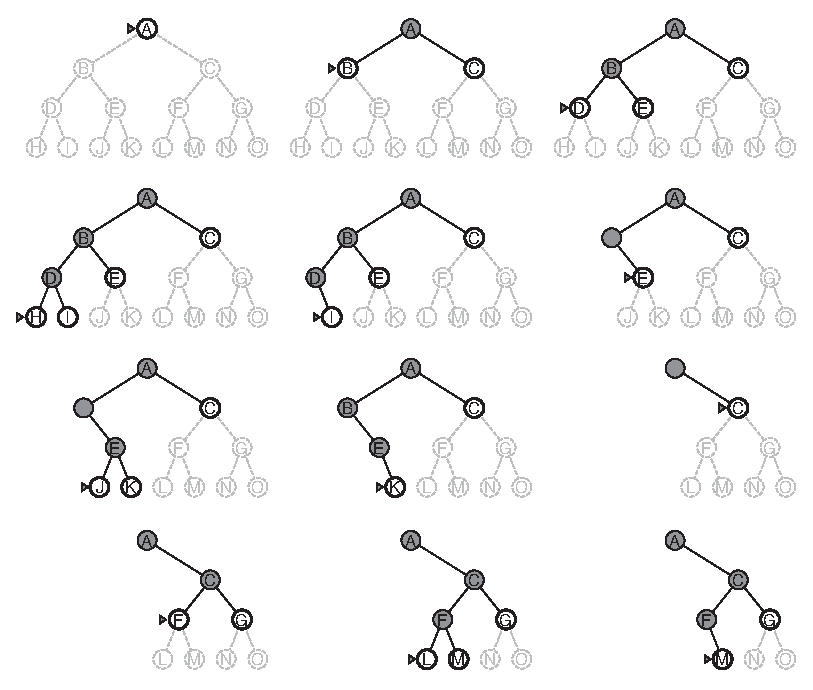
\includegraphics[width=\linewidth]{figs/dfs-progress-noblack.eps}\\
          \tiny{\href{http://aima.cs.berkeley.edu/index.html}{(Source)}}
      \end{center}
\end{frame}

\begin{frame}{Uninformed search}{Depth-first search (III)}
      Properties of depth-first search
      \begin{itemize}
        \item Completeness: No, fail in infinite-depth spaces or spaces with loops
        \item Time complexity: $O(b^{m})$, (terrible if $m>>d$)
        \item Space complexity: $O(bm)$
        \item Optimality: No
      \end{itemize}
\end{frame}

\subsection{Depth-limited search}

\begin{frame}{Uninformed search}{Depth-limited search}
      Depth-first search with depth limit L
      \begin{itemize}
        \item Nodes at depth L are not expanded
      \end{itemize}
\end{frame}

\subsection{Iterative deepening depth-first search}

\begin{frame}{Uninformed search}{Iterative deepening depth-first search (I)}
    Depth-limited search where gradually increases L
\end{frame}

\begin{frame}[plain,shrink]
      \begin{center}
          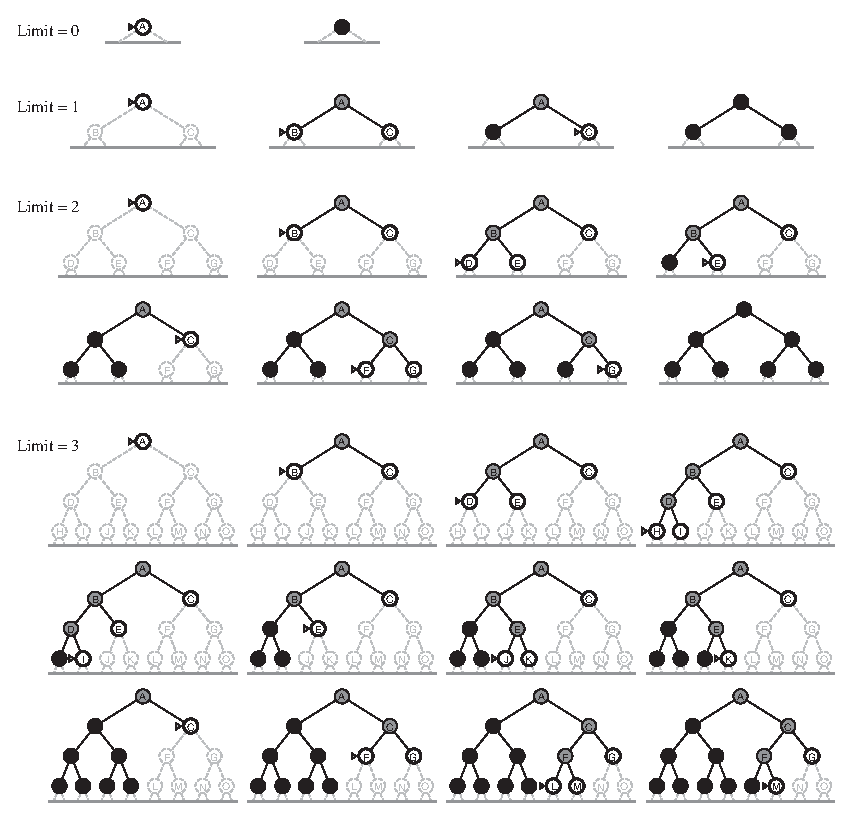
\includegraphics[width=\linewidth]{figs/ids-progress.eps}\\
          \tiny{\href{http://aima.cs.berkeley.edu/index.html}{(Source)}}
      \end{center}
\end{frame}

\begin{frame}{Uninformed search}{Iterative deepening depth-first search (III)}
      Properties
      \begin{itemize}
        \item Completeness: Yes
        \item Time complexity: $O(b^{d})$
        \item Space complexity: $O(bd)$
        \item Optimality: Yes if step cost = 1
      \end{itemize}
\end{frame}


\subsection{Comparison of uninformed search algorithms}

\begin{frame}{Uninformed search}{Comparison of uninformed search algorithms}

\begin{tabular}{cccccc}
\hline
Criterion & Breadth- & Uniform- & Depth- & Depth- & Iterative \\
          & First &  Cost & First & Limited & Deepening \\
\hline
Complete  & Yes$^*$ & Yes$^*$ & No & Yes, if $l \ge d$ & Yes \\
Time      & $b^{d+1}$ & $b^{\lceil C^*/\epsilon \rceil}$ & $b^m$ & $b^l$ & $b^d$ \\
Space     & $b^{d+1}$ & $b^{\lceil C^*/\epsilon \rceil}$ & $bm$ & $bl$ & $bd$ \\
Optimal   & Yes$^*$ & Yes & No & No & Yes$^*$ \\
\hline
\end{tabular}

\end{frame}


\section{Informed search}
\subsection{Introduction}

\begin{frame}{Informed search}{Introduction (I)}
    Use problem-specific knowledge beyond problem definition
      \begin{itemize}
        \item Best-first search
            \begin{itemize}
                \item Greedy best-first search (\textit{Búsqueda voraz})
                \item A* search
            \end{itemize}
        \item Local search algorithms
            \begin{itemize}
            \item Hill-climbing search
            \item Simulated annealing search
            \item Local beam search
            \item Genetic Algorithms 
        \end{itemize}
      \end{itemize}
\end{frame}

\begin{frame}{Informed search}{Introduction (II)}
    Best-first search
      \begin{itemize}
        \item Use an evaluation function $f(n)$ for each node
        \item Estimate of ``desirability''
        \item Expand most desirable unexpanded nodes
      \end{itemize}

    Most algorithms use a \alert{heuristic function} or just \alert{heuristic} ($h(n)$)
      \begin{itemize}
        \item Estimated cost of the cheapest path to goal
      \end{itemize}

    Special cases
      \begin{itemize}
        \item Greedy best-first search
        \item A*
      \end{itemize}
\end{frame}

\subsection{Greedy best-first search}

\begin{frame}{Informed search}{Greedy best-first search (I)}
    \begin{columns}
 	    \column{.50\textwidth}
            It only considers the heuristic
            \begin{itemize}
                \item Greedy search expands the node that \textit{appears} to be closest to the goal
            \end{itemize}

 	    \column{.50\textwidth}
            \begin{block}{Greedy search}
                $f(n) = h (n)$
            \end{block}
    \end{columns}
    
    \bigskip

    Example: Find a path between Arad and Bucharest
    \begin{itemize}
        \item Heuristic: Straight-line distance
    \end{itemize}

    \centering 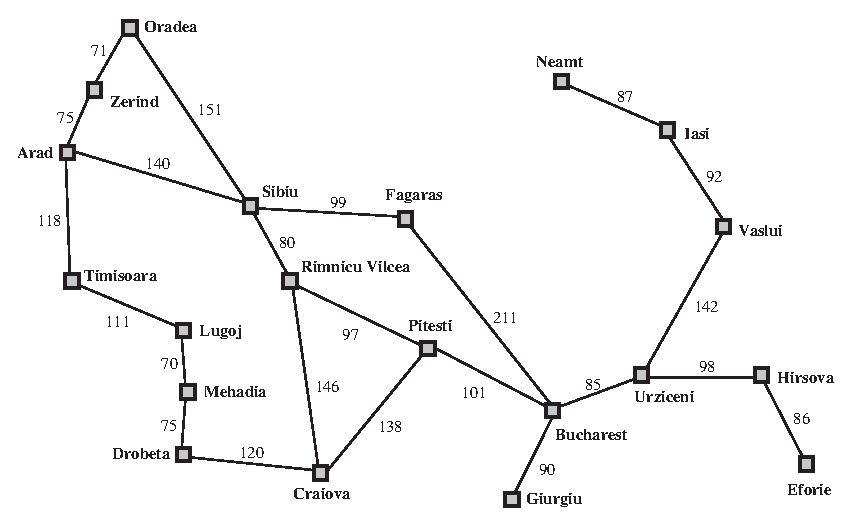
\includegraphics[width=0.6\linewidth]{figs/romania-distances.eps}\\
    \tiny{\href{http://aima.cs.berkeley.edu/index.html}{(Source)}}
\end{frame}

\begin{frame}[plain,shrink]
      \begin{center}
          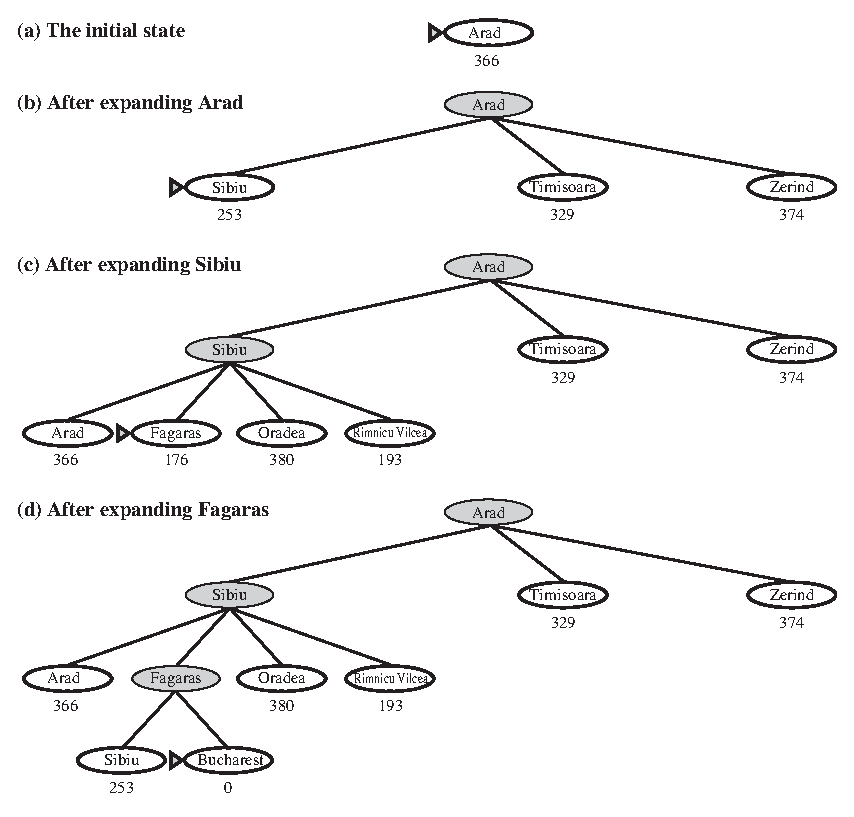
\includegraphics[width=\linewidth]{figs/greedy-progress.eps}\\
          \tiny{\href{http://aima.cs.berkeley.edu/index.html}{(Source)}}
      \end{center}
\end{frame}

\subsection{A*}

\begin{frame}{Informed search}{A* (I)}
    \begin{columns}
 	    \column{.50\textwidth}
            It considers the heuristic and the cost
            \begin{itemize}
                \item $h(n)$: Estimated cost to solution from node n
                \item $g(n)$: Cost to node n
            \end{itemize}

 	    \column{.50\textwidth}
            \begin{block}{A*}
                $f(n) = g(n) + h (n)$
            \end{block}
    \end{columns}

    \bigskip

    Theorem: A* is optimal if $h(n)$ is \alert{admisible}
        \begin{itemize}
        \item A* is admisible if it never overestimates the cost
        \item Example: Straight-line distance never overestimates road distance
        \end{itemize}
    \bigskip
\end{frame}

\begin{frame}[plain,shrink]
      \begin{center}
          \quad 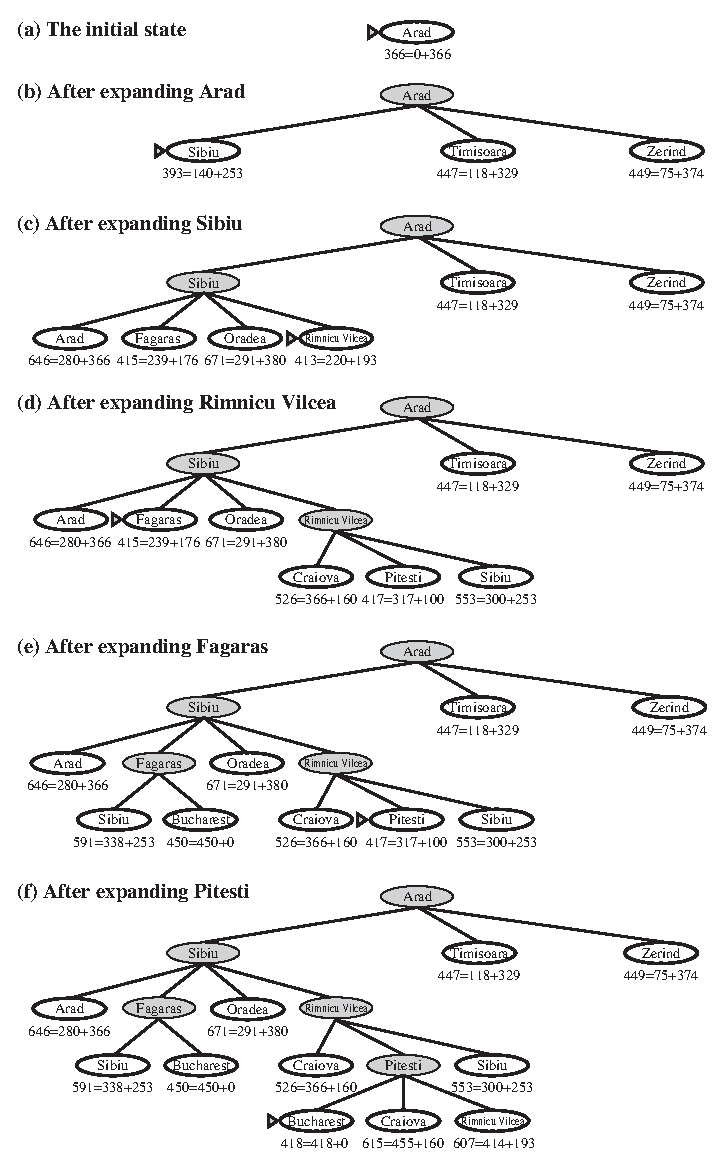
\includegraphics[width=\linewidth]{figs/astar-progress.eps}\\
          \tiny{\href{http://aima.cs.berkeley.edu/index.html}{(Source)}}
      \end{center}
\end{frame}

\begin{frame}{Informed search}{A* (III)}
      Properties
      \begin{itemize}
        \item Completeness: Yes
        \item Time complexity: Exponential
        \item Space complexity: Keeps all nodes in memory
        \item Optimality: Yes
      \end{itemize}
\end{frame}

\section{Study cases}

\begin{frame}{Study case}{Case I: Logistics?}
    TODO
\end{frame}

\begin{frame}{Study case}{Case I: GTOC?}
    TODO
\end{frame}

\end{document}
